\chapter{Implementation}
 {\color{red} the following is from the rejected paper on performance measurements (kakapo)

  It is a place holder for more text which is not ready yet....
 }
\section{BGP performance characterisation}

% % \label{sec:motivation}

\begin{figure}[h!]
	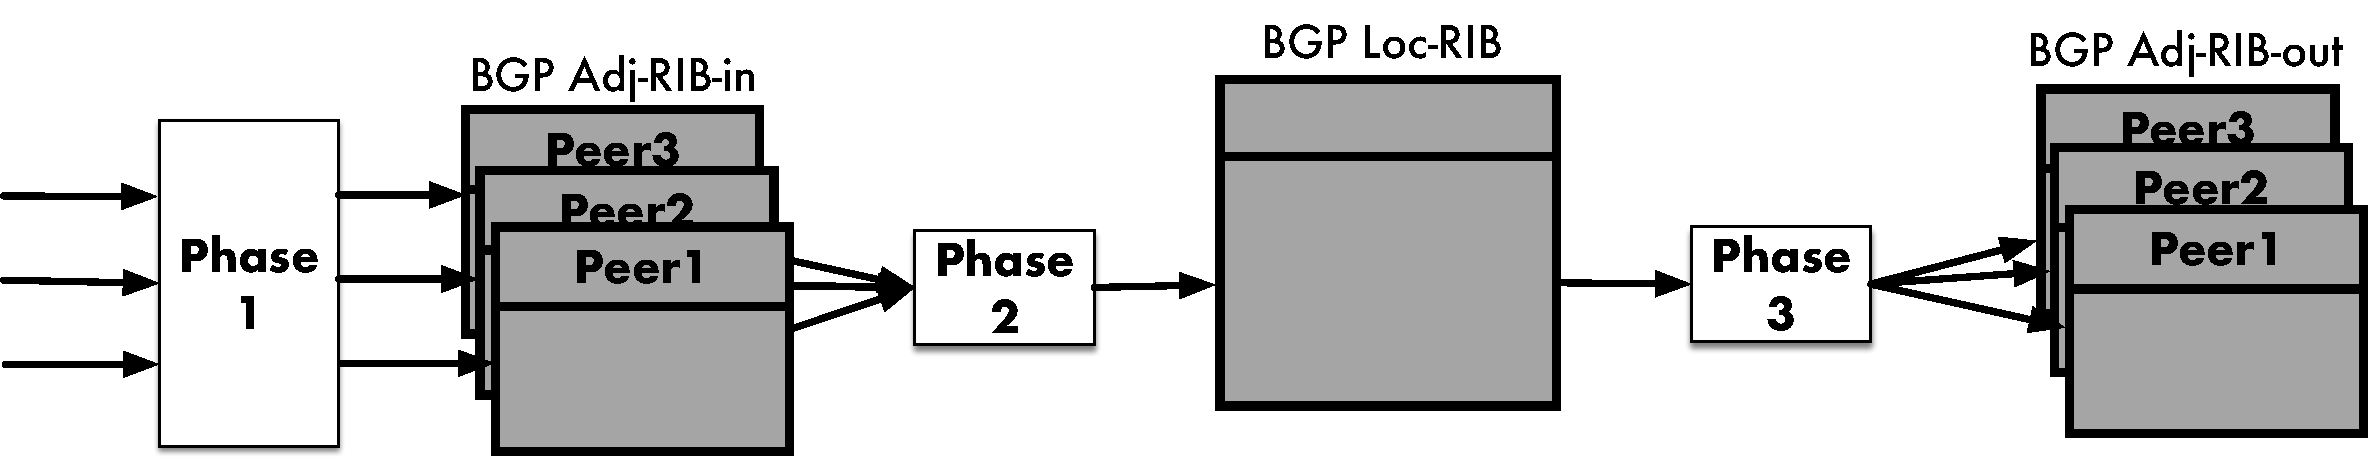
\includegraphics[width=\linewidth]{images/routeSelection.pdf}
	\caption{The BGP protocol defines a complex processing pipeline for route updates, which relies on multiple data structures to maintain intermediate information.} \label{fig:routeSelection}
\end{figure}

In this section, we briefly discuss the performance bottlenecks of a BGP speaker
and motivate the design of our system with a set of recent use-cases.
Processing route updates is the core functionality of a BGP speaker. The
processing algorithm consists of three phases, depicted in
Figure \ref{fig:routeSelection}, and precisely defined in the BGP protocol
specifications~\cite{rfc4271}. {\it Phase 1} processes, filters and rank
routes, based on the local speaker configuration. Filtered routes from each
peer are stored in the Adj-RIB-in tables, alongside intermediate processing
results and also linkage information between input route updates and main RIB
entries.  {\it Phase 2} compares all available routes for each prefix, using
Phase 1 ranking outcomes and elects a single route for each prefix.  This stage
stores its route selection results in the global BGP Loc-RIB table.  Finally,
{\it Phase 3} filters and modifies the selected routes from Phase 2 based on
peer-specific policy, potentially modifying path attributes such as
communities, AS path, MED and LocPref.
Stage 3 results are stored in per-peer Adj-RIB-out tables.

BGP speakers must maintain and manage a highly complex routing state which
expand to multiple GB of main memory in a core router. As a result, reasoning
about their performance is difficult and depends heavier on the BGP trace
characteristics. Network operators frequently revert to major investment in
specialized hardware in order to recreate realistically network conditions and
explore the impact of different tuning parameters on the speaker performance.
In parallel, the use of specialized hardware leads to limited widely acceptable
measurement standards. In order to further highlight the measurement challenges
we discuss two specific BGP use cases.

\textbf{IXP and Route Server scalability:} The increasing importance of Internet Exchange Points (IXPs) and Route Servers
(RS) leads to new scalability challenges for software BGP speakers.
RSs must support an unprecedented BGP workload including significantly larger
RIB sizes and peer numbers, as well as providing multiple independent `views'
or RIBs, each enforcing unique policies. Although IXPs employ existing open
source speakers to implement their RSs, the majority of these projects remains
single-threaded and lack the ability to easily ``scale-up'' during
high-utilization periods. Such limitation drove Google to implement Raven,
a proprietary multi-thread BGP speaker for their SDN-enabled edge peering
infrastructure~\cite{Yap2017}. Network operators require a standardized
methodology to evaluate the performance of BGP speakers under extreme load
conditions.

% Can we move these into the result section?

% The current favoured solution for this role is Bird, based on its
% rich and flexible policy configuration language and its superior performance.
% However Bird and its direct competitors FRR and OpenBGPD remain effectively
% single threaded systems \footnote{OpenBGPD implements a single separate thread
%     to manage the Route Decision Engine, however our tests indicate that this
%     provides a very small contribution to performance under stress since the
%     other threads utilisation remain low whilst the RDE engine is working at
% 100\% CPU} unable to benefit from multi-core systems: this limitation drove
% Google to implement a proprietary new highly parallel BGP speaker {\it Raven}
% for Espresso\cite{Yap2017}, Google’s SDN-based Internet peering edge routing
% infrastructure.  In this context the need to quantify the limits of performance
% and scale for Route Servers thus takes on a higher level of significance.

\textbf{Next-generation BGP speaker architecture:} A number of studies have
identified challenges in the design of BGP speakers and have proposed novel
architectures to improve their performance and flexibility. For example,
Keller \textit{et al.}\cite{Keller2010b} have proposed a virtualization architecture for
BGP speakers, that allows easy state migration,
while Grover \textit{et al.}\cite{grover2011} have developed a multi-threaded routing protocol
platform and evaluate the impact of different task scheduling approaches.
Unfortunately, the lack of a generic open-source performance evaluation does
not allow a comparison in the impact of the proposed changes in BGP protocol
processing performance.
\section{Architecture}\label{sec:arch}

Characterising BGP speaker performance entails several major challenges.
Firstly, whilst traffic generation should conform to basic BGP protocol
semantics in order to ensure interoperability, modified BGP software routers to
generate realistic traffic can incur processing overheads, limit traffic
generation capabilities and potentially introduce measurement artefacts.
Secondly, to study BGP speaker behaviour in resource poor environments requires
fine grained resource control, in order to emulate the CPU and memory
constrained processing environment available in actual network devices.
Thirdly, the measurement task still requires reasonable standards support
to accommodate a wide range of experimental scenarios.

To address these challenges we develop an holistic BGP characterisation
framework. The platform consists of two main components: {\it kakapo},
a flexible and high-precision BGP testing framework, and
	{\it Kagu}, an experiment automation tool offering precise resource control
and monitoring capabilities, using CPU virtualization technologies.  An
important supplementary component of {\it kakapo} is a lightweight BGP
relay/proxy, {\it kakapo-relay}, which allows us to characterise the baseline
performance of kakapo as a monitor and load generator.  Performance
measurements obtained from kakapo with kakapo-relay as the System Under Test
provide confidence that observed performance envelopes for BGP speakers are not
artefacts of the measurement infrastructure.  For the rest of this section we
discuss in detail the design and functionality of each component.

%\begin{minipage}[c]{.45\linewidth}
\begin{figure}
	\centering
	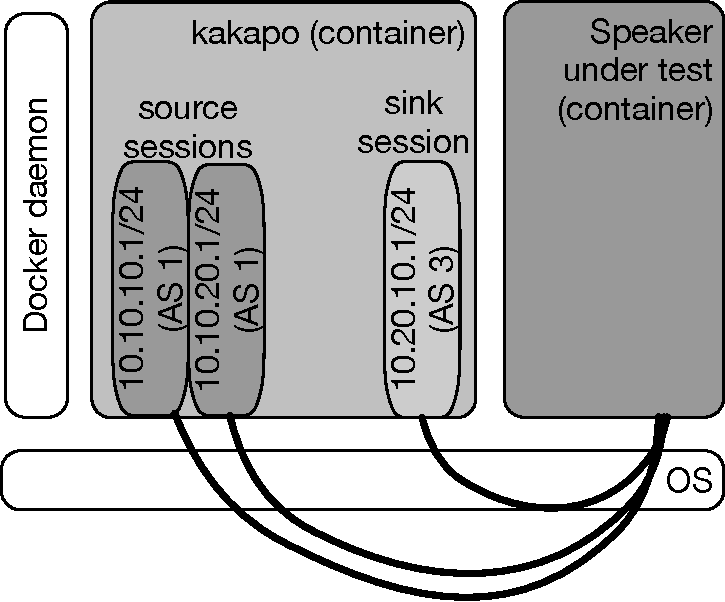
\includegraphics[width=.45\linewidth]{images/arch.pdf}
	\caption{Kakapo architecture.}\label{fig:arch}
\end{figure}

% \begin{minipage}[c]{.45\linewidth}
%     \centering
%     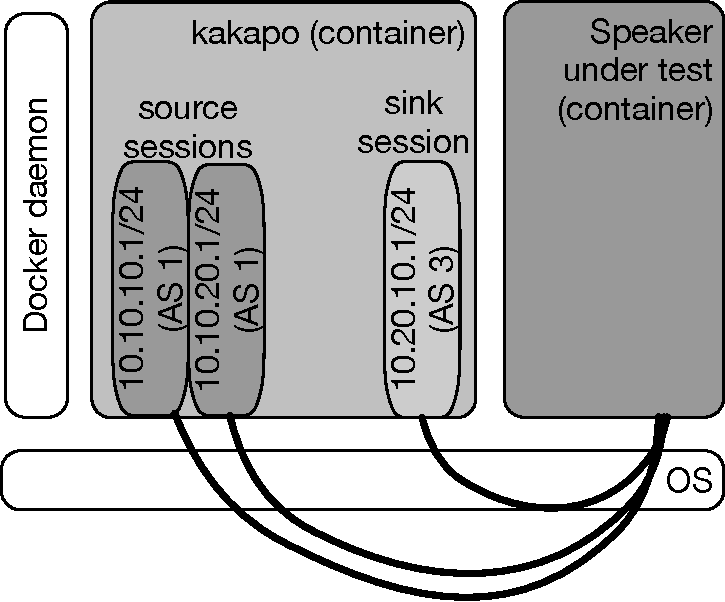
\includegraphics[width=\linewidth]{images/arch.pdf}
%     \captionof{figure}{Sample
%     sequence diagram for a bursty single-peer kakapo
% experiment.\label{fig:traffic-model}}
% \end{minipage}
% \begin{figure}
%     \centering
%     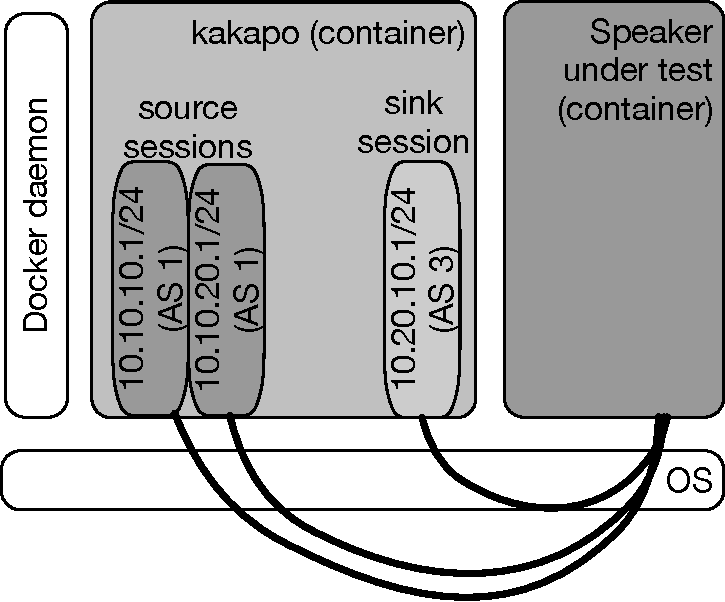
\includegraphics[width=0.5\linewidth]{images/arch.pdf}
%     \caption{Enter Caption}
%     \label{fig:enter-label}
% \end{figure}
\subsection{Kakapo: BGP performance characterisation}

% High level overview of the system
Kakapo is a high-precision BGP traffic generation and monitoring application
written in C. It is designed to measure the performance of a BGP speaker for
varying load conditions by measuring the time to process a number of BGP
messages. Kakapo uses a black-box testing approaches and relies solely on BGP
message times to understand the impact of the protocol load on the speaker
performance.  In order to perform the measurement, kakapo establishes multiple
parallel BGP sessions with a speaker and emulates the behaviour of multiple BGP
speakers. Kakapo BGP sessions are RFC-compliant, relying on a minimal complete
BGP Finite State Machine, thus allowing the test system to measure the
performance of any software and hardware router.

% Describe how things are connected
The architecture of kakapo is depicted in Figure~\ref{fig:arch}. For each
experiment kakapo establishes a single passive sink (monitor \& measurement)
session towards the speaker, and one or more source (traffic generation)
sessions, with each session configurable in terms of BGPID, AS number and
Optional Capabilities.  Each experiment commences by initialising the BGP
speaker under test (BSUT) with an empty RIB and configured to ensure that
routes received from the emulated source test peers will be imported into the
RIB and re-exported towards the destination sink test peer.  Typically, the
BSUT and sink peers are configured in the same AS (iBGP sessions) whilst the
sink peer is in a different AS, (eBGP session).  If the BSUT has a configurable
MRAI (Minimum Readvertisement Interval) timer this must be disabled to ensure
that route updates are always promptly re-announced.  As a result, every route
advertisement or withdrawal from a source session causes the speaker to
immediately transmit a corresponding route update to the sink session, once the
route has been processed.  By orchestrating both the sinks and the source
stream from a single application the system can precisely measure timestamps
and thus RTTs for each update.

% In operation kakapo implements concurrent multiple BGP speaker
% endpoints, using distinct network addresses at the same host, usually
% configured as loopbacks.

% Describe how data are generated
Kakapo allows experimenters to execute a wide range of measurement scenarios.
Firstly, the application allows an experiment to target both initial RIB population and RIB update performance, by controlling whether BGP sessions are reset between experimental runs.
Secondly, route traffic generation can either be bursty, where updates are transmitted in batches, or continuous, where route updates are transmitted continuously using a closed-loop mechanism that ensures a fixed number of updates is always in-flight.
Finally, experiments can control the number of source BGP sessions, and if more than one source are configured, to control which sessions generate route updates.

% measurement details
The principle type of measurement is the elapsed times between bursts of updates
sent by the source until the corresponding updates are all received at the
sink.  Updates are typically sent in discreet bursts, and the time taken to
send and receive these bursts is also measured, in addition to the delay
between sending and receiving.
% The BSUT is expected to be
% configured such that it imports some or all routes from the source and exports
% some or all routes to the sink.

Kakapo experiments have a three-phase lifecycle:
conditioning, main mode and termination.  During conditioning,
full route tables (Adj-RIB-In) are established for all route source
peers. During the main phase, further updates are generated however all subsequent
Updates are for prefixes which have already been announced by all peers.
As a result, the size of all RIBs is fixed, allowing
experimenters to evaluate the effect of different size route tables.
During the termination phase, all peer sessions are terminated by sending BGP
Notifications.  This phase offers the opportunity to evaluate the propagation
latency of these route withdrawal through the BSUT. Unfortunately, practical
experience developing this tool has revealed several inconsistent
BSUT behaviours and the lack of a simple mechanism to identify the `last'
withdrawal, does not allow to isolate their effects.

Continuous mode measurements are implemented by transmitting an
initial burst sequence of updates: the traffic sink accepts the resulting
Update stream and responds by transmitting additional further updates on the
source session(s) in order to maintain the in-flight quota at the
pre-configured level.  The principal objective of this test is to characterise
the continuous performance capability of the BSUT.  This requires that the
transmit `credit' window is set sufficiently large.  We observed that a value
of around 5,000 Updates was sufficient to drive all of the systems in our study
to their maximum rate, without incurring unnecessary congestion and buffering
latencies.

The traffic generation model must ensure that initial route announcement
precisely populate a set route table size, while subsequent routes announcement
are always selected by the BSUT, in order to be announced to the sink session.
In order to ensure this requirement we exploit the Local Preference attribute value.
Since Local Preference is a 32 bit value there is a possibility of wraparound
if every Update incremented LocPref, hence we only increment LocPref value when
wrapping around the complete RIB.  Thus during the initial conditioning phase
the most recent transmitting peer is always the source of preferred routes, and
the full route table is re-announced by the BSUT for each connected source
peer.

Kakapo synthesises route prefixes sequentially, using a configurable initial
seed IP address and a configurable prefix length.  Kakapo also enforces
continuous changes in AS path content (but not length), firstly because sending
duplicate routes is not permitted, and also for diagnostic purposes and to
allow future extension to individual message correlation.  Paths are also
customised based on source peer.  Customisation is based on modifying
intermediate AS numbers in the AS path.

Real world internet route tables have varying numbers of prefixes in each
update: a complete table contains typically around 750k
prefixes\footnote{{http://www.routeviews.org/peers/peering-status-by-as.html}}
and 150k distinct routes, which is an average of about 5 prefixes per unique
Path.  Kakapo produces uniform Routes with a fixed number of prefixes per Path
- in almost all of our experiments reported in this paper we use a 160k/5
profile - i.e. the full table is size is 800k with 160k distinct origin ASes.

	{\it Canary routes} is a technique used to determine when route processing has
been completed in the cases where some or all transmitted Updates are {\it not}
re-announced, and also simply for confidence that an experimental phase has
fully completed.
%This experimental mode enables measurement of an important and different distinct performance attribute to the case where all received routes are re-exported.
Since in real world operation it is often the case that received routes will
not be preferred and re-announced, it is difficult to measure this
outcome precisely due to the lack of a notice for the processing completion.
Canary routes are simply routes which are
constructed such that they will always be propagated: typically this means that
for each source peer a different unique canary prefix is defined.  By sending
a canary Update after a test burst which is not expected to be propagated we
can measure the processing delay by simply timing the delay before the canary
re-emerges.  This strategy relies on the BSUT processing routes in strict
sequence for a given peer, which must be independently confirmed for each BGP
speaker.  All of the BGP speakers in our study did exhibit this behaviour,
including those which claim or exhibit multi-threaded processing capability.
Canary routes also provide a good method for troubleshooting invalid
configurations - since kakapo currently does {\it not} correlate every
transmitted and received messages it uses simple counts of messages to
determine when a burst has been completely received.  By transmitting a canary
as the last message in a burst, kakapo can quickly detect and report when some
Updates have been dropped.

In order to evaluate the base performance of our measurement platform, the
kakapo codebase contains the kakapo-relay application, a reference BGP speaker
supporting the minimal functionality required to peer with the kakapo system.
The purpose of kakapo-relay is to provide a benchmark measure of the
performance capability of the test harness and characterise any measurement
artefact incurred by the platform. Kakapo-relay is written in C and uses iovec
and epoll to achieve low latency and line rate network throughput in realistic
BGP test scenarios.  Both kakapo and kakapo-relay optimise network performance
by working with very large buffers and executing read and write operations
which typically address very large numbers of BGP messages in a single system
call.  The continuous rate measurement design is especially sensitive to
efficiency issues: if kakapo transmits updates too quickly, it forces much
smaller messages at network Layers 2 and 3, which pushes up the CPU demand for
the target systems and results in much lower performance than would be the case
if Updates are transmitted in slightly larger blocks.  Since our objective is
to establish how fast the BSUT can perform under optimal conditions we adjust
the transmit block size parameter to ensure that TCP and Ethernet transfers are
large enough to avoid this effect (but still much smaller than the `in-flight
window').  However it should not be ignored that in many real world scenarios
routing traffic packet scheduling may not be so optimal, and thus these BGP
speakers may perform even less well than our measurements show.
% Whether
% distributing load over multiple physical interfaces would improve matters is
% a matter for further investigation.

\subsection{Kagu: BGP experiment automation}

A major challenge for network experimentation is reproducibility. Kagu is an
automation platform, built around kakapo, allowing experimenters to deploy and
parallelize the execution of BGP experiments. In parallel, kagu also automates
measurement data and logging information collection for offline processing.

OS virtualization is a key technological enabler for Kagu, which supports
integration with docker and the libvirt management library.  The docker
integration allows kagu to run kakapo and software router as docker containers
and to use docker management operations to spawn and terminate them.
Furthermore, detailed logging information are collected through the
systemd/journald services in the container. In order to run an experiment, the
platform requires as input the router and the kakapo configuration parameters
and the platform will use docker technologies to execute the experiment and
collect the results.

Furthermore, libvirt integration allows kagu to deploy large-scale experiments
with complex network topologies over a hypervisor-based virtualization
platform, like KVM. VMs derive from a base Ubuntu image with the dockerd
daemon installed and configured to exposes remote access via HTTP.

During the deployment of a multi-host experiment, kagu builds all the required
virtual links between VMs, as well as a control plane network which uses
dynamic DNS and cloud-init to map VM control interface addresses to user
friendly host names. A custom libvirt network topology provisions distinct
unique virtual network address blocks onto each VM and dynamically updates the
configuration of a local DNS server.  Finally, the framework offers an
arp-router agent which install routes to loopback and allows connectivity over
unnumbered network interfaces.

Both test harness (kakapo) and target systems are bundled as Docker images
which enables them to be easily started and stopped in remote virtual machines
using the ‘remote Docker’ feature.  Remote Docker allows standard Docker
commands, such as ‘docker run’, ‘docker kill’ and ‘docker pull’ to be executed
on arbitrary target systems from a single controlling machine  Thus a cluster
of multiple VMs having varying resource capability can easily be orchestrated
to run multiple sets of experiments in parallel.  A complementary set of
scripts (kakapo-virt) is used to create and provision the target virtual
machines.

The main system elements are:

\begin{itemize}
	\item kakapo core  a ‘C’ language BGP test tool which can act
	      as a BGP peer, operating simultaneously in both route sink and route source
	      modes
	\item kakapo relay  a ‘dummy’,‘C’ language, BGP router which allows
	      baseline calibration of the test system
	\item kakapo runner  a run-time
	      integration framework for controlling multiple test runs with ranges of
	      test parameters
	\item kakapo ingest  offline analysis of the test data
	      generated by kakapo, including on-demand gnuplot graph display
	\item
	      kakapo-virt  a VM and virtual network provisioning tool --- kakapo virt
	      creates and provisions test VMs with different resources (CPUs, RAM,..) to
	      provide execution environments for kakapo targets and test harness instance
	      to execute in.  Kakapo-virt also provisions both a control plane network to
	      allow remote orchestration of the VMs and their Docker execution
	      environment, and a separate experimental network context which meshed VMs
	      which are configured to operate as a single experimental topology
	      somewhat like mininet, but for KVM virtual machines.

	\item kagu a build and deploy system for the (mostly Dockerised) components of kakapo
	\item arproute a network utility which enables virtualised systems to discover routes between themselves without manual configuration.
	\item Docker, systemd, libvirt and nginx with webdav support --- provides the infrastructure environment in which kagu and kakapo operate
\end{itemize}

Of these components some work before a testing session (kagu, kakapo-virt), and
others after testing sessions have finished (kakapo ingest).  The core system
consists of kakapo core, kakapo relay, kakapo runner: of these kakapo runner
is the coordination tool: it schedules execution of test systems in virtual
environments, typically systems consisting of kakapo core paired with another
BGP speaker such as bird, frr (quagga), OpenBGP, hbgp, or another hardware or
software router.  Kakapo core starts and stops BGP peer sessions with the
SystemUnderTest, monitors the response performance and records the
configuration and results in test data files on a centralised storage system
for later analysis.  Kakapo runner feeds the required test parameters to kakapo
core: typically these specify a range of BGP route table sizes (two
parameters), and a cycle count for the number of repetitions of route changes
to send, updating the initial route table load.  The recorded results are delta
time measurements for the begin and end of both reception and transmission of
groups of Update messages.  Results are uploaded as structured text files to
a webdav server.

% % \subsubsection{Docker usage}

% % \subsubsection{kakapo-core}

% % \subsubsection{kakapo-relay}

% % \subsubsection{Linux TCP / kernel limitations}

% % Observations of the network behaviour of both the existing platforms such as
% % frr, bird and OpenBGP, and also the custom implementations developed for the
% % study (hbgp, kakapo and kakapo-relay) show the impact of Linux TCP
% % implementations and default configuration

% \subsubsection{Data analysis --- kakapo-ingest}

% Kakapo-ingest is an offline tool which consumes the output generated by
% kakapo-core.  Kakapo currently uses webdav as a repository access mechanism: at
% the end of every execution of a single kakapo run a text based data file is
% uploaded to a central server using webdav.  The file format captures ‘metadata’
% such as the kakapo parameters defining RIB size, update blocking factors,
% prefixes per update, as well as all significant context for the experiment,
% e..g the software router name and version, the number of cores and RAM
% allocation, the date and time of the experiment, and the ‘topic’ which is used
% to group a group of experiments which collectively define an entire
% ‘experiment’

% Kakapo-ingest is a tool whose purpose is to select and preprocess the raw data
% from multiple kakapo-core runs into a format suitable for graph plotting or
% further analysis.  K-ingest resembles an SQL query tool in that it requires
% a set of selection terms to be given which represent a filter over the total
% set of data points.  The Query syntax allows an explicit selection of
% a ‘x-axis’ variable and a separate discrete multi-line selector value set,
% combined with filter terms which define specific values which must match data
% points in order to include them.

% In operation Kakapo-ingest takes a directory path (/var/webdav in the example
% below), and recursively scans it for data files in the correct kakapo format.
% Kakapo-ingest has several modes of execution which allows the dataset to be
% queried and selection criteria defined up to the point that a coherent set of
% data points can be extracted and plotted in a gnuplot graphing environment.

% An example k-ingest query is:

% ingest /var/webdav TOPIC=RIBTEST PLATFORM=bird,frr,bgpd,hbgp RIBSIZE=?

% % In this example, a graph is defined using the metadata field ‘RIBSIZE’ as the
% control parameter (y-axis), and showing separate plots for each of the named
% platforms (bird, frr, OpenBGP, haskell BGP).  In this case there were no
% variants such as CPU count or RAM size present in the database, and so the
% query is already unambiguous and able to directly generate a gnuplot data file
% and if required plot it interactively or export to a graphic file.  Otherwise
% additional selection terms would be required, such as

% ingest \ldots CORES=4 MEMORY=8192

% The flexible query syntax enables other parameters to be plotted, for example
% a graph showing performance for different numbers of prefixes in a fixed count
% of Updates is possible simply by changing the control parameter to ‘GROUPSIZE’
% and defining a suitable range of parameters in kakapo-runner to create the
% required dataset.

\section{Characterising BGP speaker performance}\label{sec:result}

To demonstrate the capabilities of the kakapo and kagu systems we conduct
a performance analysis of a representative set of production software BGP speakers.
Specifically, using a virtualised server testbed (\S~\ref{sec:testbed}), we evaluate the
single and multi-session performance.

\subsection{Measurement setup}\label{sec:testbed}

Presently, network managers have access to a wide-range open-source BGP projects
with carrier-grade protocol support. FRR~\cite{frr} is a multi-protocol routing suite
with support for BGP. The codebase is an active fork of the Quagga project and
this speaker software is widely deployed in IXP infrastructures, as a route
server . Additionally, the code is used by white-box
vendors to provide routing protocol capability for BGP and other protocols in the control plane of their network devices.
BIRD~\cite{bird} is another widely used BGP speaker, considered to offer consistent performance,
and a rich configuration paradigm. BIRD has recently undergone a major
rewrite to integrate simultaneous IPv4 and IPv6 support, thus in our analysis we include both
version 1.6 and 2. In our analysis we also include OpenBGPD~\cite{openbgpd},
an minimal open-source BGP speaker maintained by
the BSD community, offering an alternative stable and secure BGP protocol support. Finally,
in our analysis we include GoBGP~\cite{gobgp}, a multi-threaded BGP speaker written in Go.
GoBGP proposes to capitalize on the parallelization capabilities of the GO language to provide high-performance BGP
support. However, the choice of a high-level language, in comparison to
other BGP implementation written in C, exhibits interesting challenges for overall
system performance. In our measurement study we employ FRR (v7.0), BIRD
(v1.6.6), BIRD2 (v2.0.4), OpenBGPD (v6.5) and GoBGP (v2.6.0).  All BGP speakers are
configured so as {\it not} to export routes to the local FIB.

Using kakapo we develop four representative tests. Firstly, we measure the
latency to perform a {\tt table transfer} of 800k routes. Table transfer are
a common event in the global Internet, which can significantly increase the
load of a BGP speaker and increase latency~\cite{Cheng2011}. Secondly, we measure
the latency to process a burst of 50k {\tt route updates}. Large burst of route
updates is a common effect during route instability incident. Finally, we
develop a simple rate estimation measurement to evaluate the multi-session
scalability of speakers. Specifically, kakapo develops a close loop traffic
generation mechanism, that synchronises route transmissions from a source with
route advertisement on the sink session and target to maintain a constant number
of route update in-flight at any point in time. By conducting an exhaustive
analysis of many possible window sizes for this measurements, we concluded in
using a window size of 5k routes for all platform measurements. This window
size creates a significant load on the BGP speaker, but does not result in
congestion. Using the aforementioned measurement scenario, we measure in
a multi-session setup both the average {\tt single-session burst rate} (a
single session generates the update stream) and {\tt multi-session burst rate}
(all sessions generate in parallel updates), when transmitting a continuous
update stream for a statistically significant amount of time (30 seconds).

All our tests are executed on a Dell server, equipped with two E5-2690 Intel Xeon
CPUs (2x24 Cores) with 320GB of RAM and an Intel X540-AT2 10~GbE Copper
card. All experiments are executed using docker containers. To ensure
representative high routing link performance we configure kakapo and the BGP speaker to transmit their
updates over a loopback link between two ports of a 10G NIC.

% \subsection{Single-session performance} \label{sec:single-peer}

% \input{single-host-tbl}

In order to establish a set of baseline measurement profiles, in this section
we focus our performance analysis on the single session scenario using the
metrics discussed in the previous section.  Our measurement results are
presented in Table \NH{XXX?}, reporting the mean and the standard
deviation of each measurements across 50 runs. In order to demonstrate the low
measurement overhead of our platform, the table reports additionally the
performance measurements of our custom BGP relay implementation. The relay BGP
speaker completes the table transfer in less than 90msec, while the processing
of the route updates complete in approx. 30 msec. This measurements suggest
that the impact of our measurement in the overall latency measurement is less
than 10\%. In parallel, our system generates 4x more updates than the BIRD2
speaker can process, the fastest BGP speaker in this measurement.

Furthermore, our measurement highlight that there is a significant latency
difference between a table transfer and a route update for most speakers. This
can be attributed to the significant number of memory allocations that the
speaker needs to perform in order to create the required state for each new route.

In terms of performance, we highlight that BIRD2 achieves the best performance
across all metrics. In addition, BIRD2 exhibits a non-negligible performance
improvement in comparison to BIRD. Specifically, BIRD2 processes 100 msec
faster on average the table transfer and the route update and its average
processing rate is improved by 15\%. FRR is significantly slower than BIRD and
BIRD2, especially for the average processing, which is 4x time slower in
comparison to BIRD2. Nonetheless, from a network manager perspective, FRR
supports series of configuration options, not available in BIRD. OpenBGPD
performance is measured to be somewhere between the two systems. Finally, GoBGP
exhibits the worst performance in comparison to the rest of the BGP speakers.
During our measurements we note that the GoBGP process was saturating 6 CPU
cores, which suggests that the speaker was using effectively its multi-thread
capabilities. The measurement results suggest that the use of a high-level
language (Go) can have an impact on the performance of a BGP speaker, due to
features like automated garbage collection,
while enabling multi-thread support in a BGP speaker is not guaranteed to
improve overall performance.

\subsection{Multi-session performance} \label{sec:multi-peer}

The increasing growth in IXP membership and the deployment of route server
services introduces novel scalability requirements for BGP speakers.
Motivated by this observation in the section we aim to explore the impact of
the number of active sessions on BGP speaker performance.

In order to perform this measurement, we use the ability of kakapo to establish
multiple sessions towards a speaker and measure the average processing latency
of a table transfer (Figure~\ref{fig:tbl-transfer-scalability}) and a 50k route
update batch (Figure~\ref{fig:ssbt-scalability}) for a varying number of active
BGP sessions.
Furthermore, we extend our rate estimation experiment and
consider two new scenarios: the route updates are sent over a single session
(Figure~\ref{fig:ssrt-scalability}) or the route updates are sent in parallel
from all sessions (Figure~\ref{fig:msrt-scalability})~\footnote{In this measurement, we omit GoBGP from Figure~\ref{fig:tbl-transfer-scalability}, because the latency was extremely high and present results for up to 10 active sessions in all other figures, since the speaker kept resetting BGP session for higher session numbers}.

\begin{minipage}[c]{.49\linewidth}
	\centering
	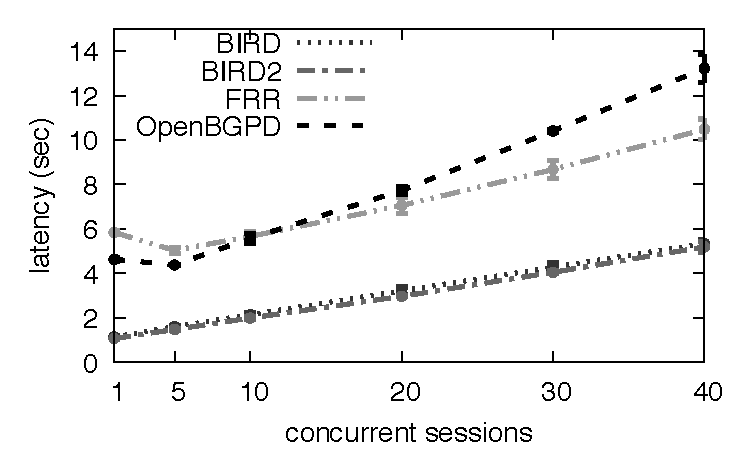
\includegraphics[width=\linewidth]{images/table-transfer-scalability.pdf}
	\captionof{figure}{Table transfer latency (800k).}\label{fig:tbl-transfer-scalability}
\end{minipage}
\begin{minipage}[c]{.49\linewidth}
	\centering
	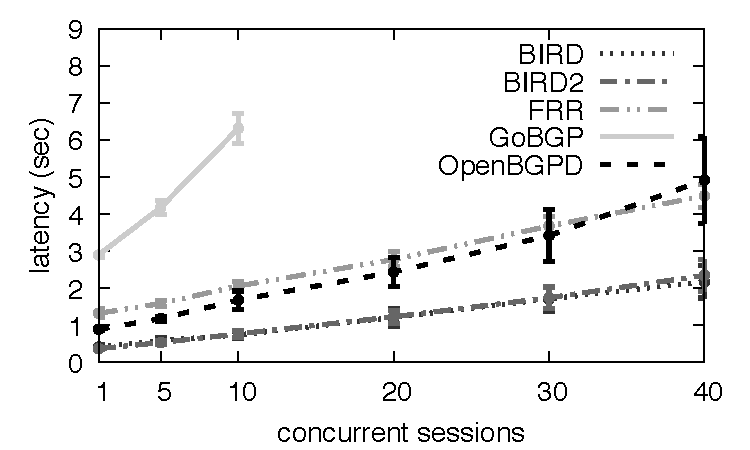
\includegraphics[width=\linewidth]{images/ssbt-scalability.pdf}
	\captionof{figure}{Route update latency (50k). } \label{fig:ssbt-scalability}
\end{minipage}

\hfill

\begin{minipage}[c]{.49\linewidth}
	\centering
	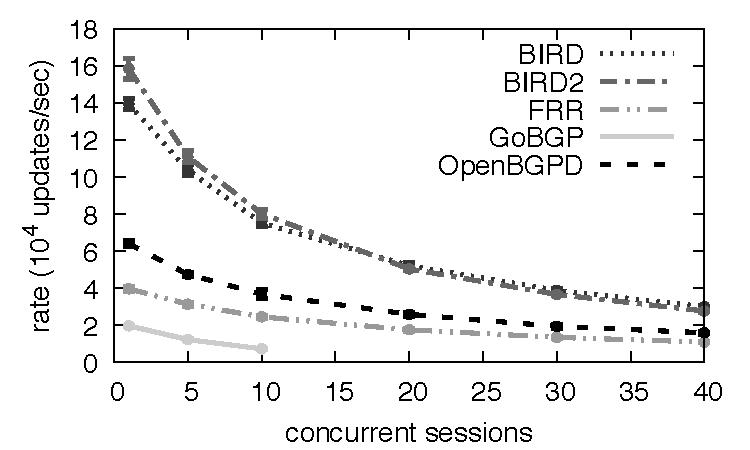
\includegraphics[width=\linewidth]{images/ssrt-scalability.pdf}
	\captionof{figure}{Single-session burst rate.}\label{fig:ssrt-scalability}
\end{minipage}
\begin{minipage}[c]{.49\linewidth}
	\centering
	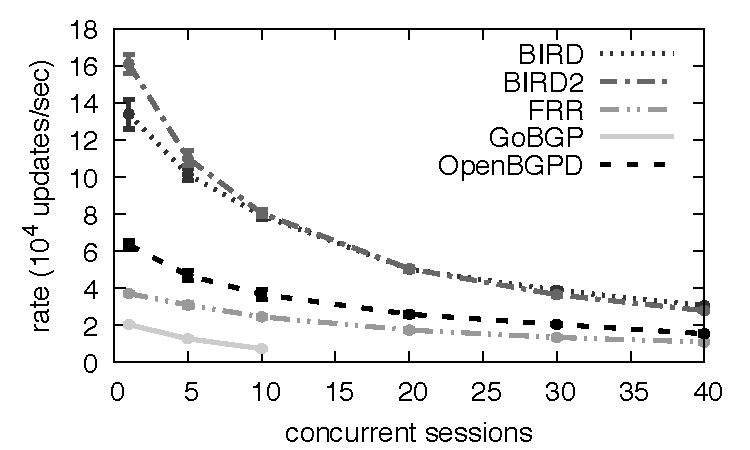
\includegraphics[width=\linewidth]{images/msrt-scalability.pdf}
	\captionof{figure}{Multi-session burst rate.} \label{fig:msrt-scalability}
\end{minipage}
\vspace{1em}

Firstly, we highlight that all speakers exhibit a very significant performance reduction as
the number of active sessions increases. This behaviour is consistent in
table transfer, update burst and continuous rate measurement scenarios.
BIRD and BIRD2 appear to experience a significant processing rate reduction for high sessions numbers, since their processing rate halves as we increase the number of sessions from 1 to 10.
Nonetheless, this performance impact is not similar in the latency measurement and both speakers exhibit a sub-linear performance decrease.
OpenBGPD and FRR exhibit a sub-linear decrease in their performance for both latency and rate measurements. These characteristics might be explained either by the employed lookup structures, which increases its lookup times for large route counts, or the internal processing scheduling mechanism.
Secondly, for all BGP speakers BGP performance varies only slightly when route updates are spread across multiple sessions.
Across all speakers there a minor performance decrease on the order to 1\%-2\% on the average route processing rate. This highlights that while all systems manage gracefully large update bursts coming from multiple parallel sessions, such as may occur during major route instabilities, however none of them manage to leverage the opportunity for parallelization to actually improve performance.
\section{Related Work}\label{sec:related}

BGP performance is a well studied problem by the measurement community.  The
majority of the studies focuses primarily on understanding the protocol-related
impact in performance critical situations, like route flapping, and only
a small set of studies have explored the BGP speaker performance
characteristics.
One of the first measurement studies on the topic~\cite{Agarwal2004}, correlated SNMP CPU route data and RouteViews dumps to
measure the data plane performance of production edge routers. Their analysis
concluded that on average BGP processing consumes approximately 60\% of the
total CPU utilization, and that a strong correlation existed between
significant CPU spikes and major BGP incidents, like the SQL Slammer worm outbreak.

Specific to the topic of performance characterisation, the IxNetwork platform
offers commercial support for BGP protocol compatibility and performance
testing \cite{ixia2004}. Using the Ixia traffic generator, Jasinska and
Malayter \cite{Jasinska2010} demonstrated significant variability in CPU
utilization between production software BGP speakers. Of great relevance to our
effort, Feldmann \textit{et al.}\cite{feldmann2004} presented a multi-dimensional study on
the factors affecting production BGP routers. Using a custom testbed equipped
with hardware-accelerated traffic generating and capturing devices, they study
the impact of the background CPU, the session count and the BGP load on the
processing latency of individual messages. Their results highlighted that the
BGP processing performance of a hardware router can increase in the order of
seconds. Similarly, Wu \textit{et al.}\cite{wu2007} developed a series of BGP interaction
scenarios to measure the impact of control and data traffic on the performance
of the BGP speaker across different platforms (CPU, NPU, ASIC).  Unfortunately,
in both studies the measurements offer limited reproducibility, since they rely
on hand-crafted measurement scenarios and specialized hardware.
